

\documentclass[letterpaper]{article}

\usepackage{hyperref}
\usepackage{geometry}
\usepackage{xspace}
\usepackage{graphicx}
\usepackage[T1]{fontenc}
\usepackage[sc,osf]{mathpazo}
\usepackage{amsmath}

\def\name{Jose Ignacio Castelli}
\def\footerlink{https://github.com/JicLotus/CV}

% PDF metadata
\hypersetup{
  colorlinks = true,
  urlcolor = black,
  pdfauthor = {\name},
  pdfkeywords = {android, software development, algorithms, computer science, mathematics},
  pdftitle = {\name: Curriculum Vitae},
  pdfsubject = {Curriculum Vitae},
  pdfpagemode = UseNone
}

\geometry{
  body={6.5in, 8.5in},
  left=1.0in,
  top=1.25in
}

% Page headers
\pagestyle{myheadings}
\markright{\name}
\thispagestyle{empty}

% Custom section fonts
\usepackage{sectsty}
\sectionfont{\rmfamily\mdseries\Large}
\subsectionfont{\rmfamily\mdseries\itshape\large}

% Don't indent paragraphs.
\setlength\parindent{0em}

% Make lists without bullets
\renewenvironment{itemize}{
  \begin{list}{}{
    \setlength{\leftmargin}{1.5em}
  }
}{
  \end{list}
}

\newenvironment{no-indent-itemize}{
  \begin{list}{}{
    \setlength{\leftmargin}{0em}
  }
}{
  \end{list}
}

\def\tilde{$\scriptstyle\sim$}
\def\bullet{$\circ$\xspace}

\begin{document}

{\huge \name}



\bigskip
\begin{minipage}{0.45\linewidth}
  \begin{tabular}{llll}
    
    
    Email: & \href{mailto:joseignaciocastelli92@gmail.com}{\tt joseignaciocastelli92@gmail.com} \\
     
    
    Github: &\href{http://github.com/jiclotus}{\tt http://github.com/jiclotus}\\
    
    Linkedin: &\href{https://www.linkedin.com/in/jose-ignacio-castelli-138763b0/}{\tt https://www.linkedin.com/in/jose-ignacio-castelli-138763b0/}\\
    
    Languages: & \textsc{en}, \textsc{es}\\
    Birth Date: & \textsc{07-18-1992}
    
    
  \end{tabular}
\end{minipage}


\hfill 
\smash{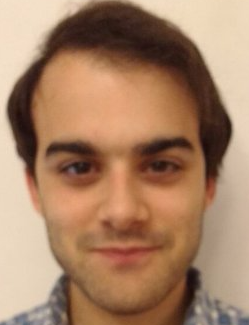
\includegraphics[width=3cm,height=3.5cm]{profilePic.png}}


\section*{Education}
\begin{no-indent-itemize}
  \item\bullet At the edge of 24 I hold a degree in Software Engineering from University of Buenos Aires 2011-2016 ( It is a 6-year university course equivalent to a Bachelor's and Master's degree) 
  \item\bullet GPA: 7.11 of 10.0
\end{no-indent-itemize}


\section*{Employment}
\begin{no-indent-itemize}


    \item \textsc{Game Development at LocalStrike and NRG Games} | Jan 2007 - Jul 2008
    \begin{itemize} \item\bullet
    I had a game sponsor called LocalStrike for my Argentum Online 2D Game Project.
    \item\bullet My Second experience with another game Sponsor(NRG Games) in the development of Argentum Online 2D project. 
    \item\bullet Vb6, Dx7,Dx8 and Mysql
    \end{itemize}
    
    
    \item\textsc{Game Development at InmortalAO} | Dec 2011 - Jul 2014
    \begin{itemize} 
    \item\bullet
    This game was online with 167 players simultaneously. Now the game status is offline; however, it is under development.
    \item\bullet \href{https://www.facebook.com/InmortalAO/}{https://www.facebook.com/InmortalAO/} 
    \item\bullet https://github.com/JicLotus/InmortalAO-CPlusPlus
    \item\bullet https://github.com/JicLotus/InmortalAO-CSharp
    \item\bullet Dx11, C++, C\# .Net , MongoDB and Mysql
    \end{itemize}


    \item \textsc{C\# QR App} | Sep 2015 - May 2016
    \begin{itemize} 
    \item\bullet  This project was developed for coil control for a recycling plant. 
    \item\bullet C\# .Net FrameWork, Php, JAVA and Android. 
    
    \item\bullet
    \href{https://github.com/JicLotus/Control-Sistematico-QR}{https://github.com/JicLotus/Control-Sistematico-QR}
    
    \end{itemize}


    \item\textsc{C\# .Net Developer at RS} | Jan 2017 - Present
    \begin{itemize}
    \item\bullet Billing management system for Supervielle Bank
    \item\bullet We use Jenkins for CI and scripts in powershell for automatic deploy
    \item\bullet  C\# , .Net framework , MSSQL, SOAP, and JS.
    \end{itemize}
    


\end{no-indent-itemize}


\section*{Projects}
\begin{no-indent-itemize}
    
    \item \textsc{3D WebGL Graphic Scene} | May 2016 - Jun 2016
    \begin{itemize}
    \item\bullet 3D graphic scene developed in WebGL and JS.
    \item\bullet Each vertex point in the graphic scene was positioned mathematically
    \end{itemize}
    \begin{itemize}
    \item \href{https://github.com/JicLotus/3DGraphicScene}{https://github.com/JicLotus/3DGraphicScene}
    
    \end{itemize}

    \item \textsc{C++/Android Dropbox Open Source} | Aug 2015 - Dec 2015
    \begin{itemize}
        \item\bullet Dropbox open source for Android.
        \item\bullet The web server was developed in RocksDB in C++ language.
        \end{itemize}    
    \begin{itemize}
        \item \href{https://github.com/JicLotus/Dropbox-source}{https://github.com/JicLotus/Dropbox-source}
    \end{itemize}

    \item \textsc{Capacitive touch sensors} |  Apr 2015 - Jul 2015

    \begin{itemize}
        \item\bullet Two capacitive touch sensors using an Atmega88pa microcontroller. These sensors were used for the control of intensity of a 12V light.
         
         \href{https://github.com/JicLotus/Capacitive-Sensor}{https://github.com/JicLotus/Capacitive-Sensor}
    \end{itemize}

\end{no-indent-itemize}

\section*{Skills}
\begin{no-indent-itemize}
    
    \item\textsc{Senior Experience}:
    \begin{itemize}
        \item\bullet \underline{Languages}: C\# .Net Framework, C++, C, SQL
        \item\bullet \underline{DB}: Mysql, MSSql
    \end{itemize} 
    \item \textsc{Semi Sr Experience}:
    \begin{itemize}
        \item\bullet \underline{Languages}: JAVA, Python, Php, Android and JavaScript
        \item\bullet \underline{DB}: MongoDB and RocksDB
        \item\bullet \underline{Video Games Api}: DirectX, OpenGL, WebGL, SDL, XNA
        \item\bullet \underline{Frameworks}: Laravel
        \item\bullet \underline{Web Servers}: IIS and Apache.
    \end{itemize}     
    \item \textsc{Jr Experience}:
    \begin{itemize}
        \item\bullet \underline{Languages}: GO
    \end{itemize}      

\end{no-indent-itemize}



\section*{Extracurriculars}
\begin{no-indent-itemize}
    \item\bullet Since I was thirteen years old I have been developing video games and company management systems in different languages. 
    \item\bullet I love playing the drums in my free time. I've played them since I was thirteen years old; however,  as I love learning informatic news every time I don't have much time to play.
\end{no-indent-itemize}






\bigskip
\begin{center}
  \begin{footnotesize}
    Last updated: \today \\
    \href{\footerlink}{\texttt{\footerlink}}
  \end{footnotesize}
\end{center}

\end{document}
